\chapter{Scattering simulation}
\label{scattering}
Finally after all our hard work of investigating the dispersion curves of
different lattices as well as finding out how to perturb them such that we form
a bandgap, we will actually simulate how a wave of a certain frequency
propagates and scatters through a finite portion of one of our lattices.

Similarly to how we joined cells together to from a strip, we will do the same
and join strips to form a finite lattice. We may then reframe our eigen-problem
systems in reciprocal space into linear systems in physical space. From there,
we can solve the linear systems to see how the energy or wave moves throughout
the entire space. All we need to do is pick a frequency for the wave we want to
simulate as well as where we want the source of excitation to be.

From the dispersion relations, we know which frequency waves are able to
propagate across the lattice and which frequencies are not transmitted through
the lattice. As we have discussed before in Chapter \ref{formstrip}, we know
that there are certain frequencies which are only able to propagate along the
interface of the strips and not anywhere else in the lattice. These are the
frequencies which we will be simulating.
%TODO: Different shape of lattices to bend waves?

\section{Our linear system in physical space}
Before we can run our scattering simulations, which essentially is solving for
the displacements of masses in our finite lattice, we need to form the system
to solve. This actually turns out to be really similar to the eigen-problems we
had earlier (albeit with a much larger matrix involved!).

The key idea in this is that we can pick and choose the frequency, $\Omega$,
and so by just
%TODO: Finish derivation of linear system

\section{Simulation results}
We can run our simulations for another frequency we want, but we know from our
dispersion relations that most frequencies will just propagate throughout the
lattice and so we would not get any discernible patterns of movement. An
example can be found in Figure~\ref{fig:randscat}.

%TODO: Add figure of scattering with uninteresting frequency

As we are interested in being able to direct waves to our liking, it is much
more exciting to fire a frequency which is only able to travel along the
boundary.

%TODO: Add figure of scattering along straight boundary

From this, it is only natural to wonder if we can shape the boundary however we
like and get it to propagate just as well.

%TODO: Add figure of scattering with bentr boundary

\subsection{2d hexagonal lattice}
\begin{figure}[!h]
\centering
\includegraphics[width=0.8\textwidth]{imgs/hexfinitemodel.png}
\caption{\label{fig:kagomeM} Schematic view of the finite hexagonal lattice
  formed from the joining of strips side-by-side, where the strips themselves
  are formed from two different halves as in Chapter \ref{perturbed}. Note the
  conditions imposed at the boundaries (masses at boundaries have no
  connections outside the lattice).}
\end{figure}

\subsection{2d kagome lattice}
\begin{figure}[!h]
\centering
\includegraphics[width=0.8\textwidth]{imgs/kagomefinitemodel.png}
\caption{\label{fig:kagomeM} Schematic view of the finite kagome lattice formed
  from the joining of strips side-by-side, where the strips themselves are
  formed from two different halves as in Chapter \ref{perturbed}. Note the
  conditions imposed at the boundaries (masses at boundaries have no
  connections outside the lattice).}
\end{figure}


